\documentclass[aspectratio=169,11pt]{beamer}

% ============================================================
% PACKAGES
% ============================================================
\usepackage{graphicx}
\usepackage{tikz}
\usetikzlibrary{positioning,arrows.meta}
\usepackage{xcolor}
\usepackage{booktabs}
\usepackage{tabularx}
\usepackage{array}
\usepackage{ragged2e}
\usepackage{hyperref}

% ============================================================
% COLORS - SAME AS PHASE-I
% ============================================================
\definecolor{GEUBlue}{RGB}{20,55,105}
\definecolor{GEULightBlue}{RGB}{238,244,251}
\definecolor{GEUGrey}{RGB}{90,90,90}
\definecolor{GEULightGrey}{RGB}{245,246,248}

% ============================================================
% BEAMER SETTINGS
% ============================================================
\usetheme{default}
\setbeamertemplate{navigation symbols}{}
\setbeamertemplate{blocks}[rounded][shadow=false]

\setbeamercolor{normal text}{fg=black,bg=white}
\setbeamercolor{frametitle}{fg=GEUBlue}
\setbeamercolor{structure}{fg=GEUBlue}
\setbeamercolor{block title}{fg=GEUBlue,bg=GEULightBlue}
\setbeamercolor{block body}{fg=black,bg=GEULightBlue}

\setbeamerfont{frametitle}{size=\Large,series=\bfseries}

% ============================================================
% LOGO
% ============================================================
% Upload the Graphic Era logo with this filename to Overleaf.
\newcommand{\GEULogo}{graphicera_logo.png}

% ============================================================
% HEADER
% ============================================================
\setbeamertemplate{headline}{%
  \begin{tikzpicture}[remember picture,overlay]
    \node[
        anchor=north east,
        xshift=-0.30cm,
        yshift=-0.12cm
    ] at (current page.north east)
    {\includegraphics[height=0.62cm]{\GEULogo}};
  \end{tikzpicture}
  \vspace{0.72cm}
}

% ============================================================
% FRAME TITLE
% ============================================================
\setbeamertemplate{frametitle}{%
  \vspace{0.03cm}
  \insertframetitle\par
  \vspace{0.04cm}
  \textcolor{GEUBlue}{\rule{\textwidth}{0.9pt}}
  \vspace{0.03cm}
}

% ============================================================
% FOOTER
% ============================================================
\setbeamertemplate{footline}{%
  \leavevmode
  \hbox{%
  \begin{beamercolorbox}[
      wd=.82\paperwidth,
      ht=0.32cm,
      dp=0.10cm,
      leftskip=.3cm
  ]{author in head/foot}
    \tiny Department of Computer Science \& Engineering |
    Graphic Era (Deemed to be University)
  \end{beamercolorbox}%
  \begin{beamercolorbox}[
      wd=.18\paperwidth,
      ht=0.32cm,
      dp=0.10cm,
      rightskip=.3cm
  ]{date in head/foot}
    \hfill\tiny\insertframenumber/\inserttotalframenumber
  \end{beamercolorbox}}
}

% ============================================================
% CUSTOM COMMANDS
% ============================================================
\newcommand{\smallnote}[1]{%
\vspace{0.08cm}
{\scriptsize\color{GEUGrey}#1}
}

\newcommand{\placeholder}[1]{%
\textit{\color{GEUGrey}#1}
}

% ============================================================
% DOCUMENT INFORMATION
% ============================================================
\title{\textbf{Project-Based Learning}\\[2mm]\large Phase-II Evaluation}
\author{\textbf{VitalRoute}\\Team ID: DSCPP-III-2026-T120}

\institute{
Department of Computer Science \& Engineering\\
Graphic Era (Deemed to be University), Dehradun
}

\date{Academic Session 2026--27}

% Marker for details that depend on the real repository / demo run.
\definecolor{FillMe}{RGB}{176,58,46}
\newcommand{\fillme}[1]{{\color{FillMe}\bfseries [#1]}}
\definecolor{PassGreen}{RGB}{28,116,52}
\newcommand{\pass}{{\color{PassGreen}\bfseries Pass}}
\newcommand{\fail}{{\color{FillMe}\bfseries Fail}}

% ============================================================
% DOCUMENT
% ============================================================
\begin{document}

% ============================================================
% SLIDE 1 - TITLE
% ============================================================
\begin{frame}[plain]
\begin{tikzpicture}[remember picture,overlay]
\draw[GEUBlue,line width=3pt] (current page.north west) -- (current page.north east);
\node[anchor=north east,xshift=-0.45cm,yshift=-0.35cm] at (current page.north east)
{\includegraphics[height=1.0cm]{\GEULogo}};
\node[align=center,text width=.84\paperwidth] at ([yshift=.25cm]current page.center)
{
{\color{GEUBlue}\fontsize{26}{30}\selectfont\bfseries PROJECT-BASED LEARNING}\\[3mm]
{\fontsize{18}{22}\selectfont PHASE-II EVALUATION}\\[7mm]
{\color{GEUGrey}\Large\bfseries ML-Core: A C++-Based Implementation of Fundamental Machine Learning Algorithms}\\[3mm]
{\color{GEUBlue}\normalsize Team ID: DSCPP-III-2026-T170}
};
\node[align=center,anchor=south,yshift=.42cm] at (current page.south)
{
\bfseries
Department of Computer Science \& Engineering\\
Graphic Era (Deemed to be University), Dehradun\\[-1mm]
\scriptsize Academic Session 2026--27
};
\end{tikzpicture}
\end{frame}

% ============================================================
% SLIDE 2 - TEAM
% ============================================================
\begin{frame}{Team \& Mentor Details}
\begin{columns}[T,totalwidth=\textwidth]
\column{.48\textwidth}
\begin{block}{Team Information}
\begin{tabular}{@{}ll@{}}
\textbf{Team ID:} & DSCPP-III-2026-T170\\
\textbf{Semester:} & 3rd\\
\textbf{Sections:} & ML2, DS1, DS2\\
\textbf{Domain:} & Machine Learning\\
\end{tabular}
\end{block}

\column{.48\textwidth}
\begin{block}{Team Members}
\footnotesize
1.\quad Shubhangani Kotiyal -- 2510370294 \emph{(ML2)}\\
2.\quad Ishanaya Agarwal -- 2510380249 \emph{(DS1)}\\
3.\quad Harshita Joshi -- 2510380118 \emph{(DS2)}
\end{block}
\end{columns}

\vspace{2mm}

\begin{block}{Mentor}
Dr.Hriday Kumar Gupta
\hfill
\textbf{Interactions completed:} 3
\end{block}
\end{frame}

% ============================================================
% SLIDE 3 - PHASE-I RECAP
% ============================================================
\begin{frame}{Phase-I Recap \& Feedback Incorporated}
\begin{block}{Phase-I Status}
\footnotesize
In Phase I, ML-Core focused on planning the implementation of six fundamental machine learning algorithms: Linear Regression, SVM, KNN, K-Means, Hierarchical Clustering, and PCA. The team studied their mathematical foundations, defined the project objectives, and assigned two algorithms to each member. The initial proposal used C, with coding and testing planned for Phase II.
\end{block}

\vspace{2mm}

\begin{columns}[T,totalwidth=\textwidth]
\column{.48\textwidth}
\textbf{\color{GEUBlue}Feedback Received}
\begin{itemize}\itemsep2pt
\footnotesize
\item Use C++ to demonstrate object-oriented programming concepts.
\item Move from theoretical planning to working algorithm implementations.
\item Add dataset input and validate results using suitable test cases.
\end{itemize}

\column{.48\textwidth}
\textbf{\color{GEUBlue}Changes Incorporated}
\begin{itemize}\itemsep2pt
\footnotesize
\item Changed from C to C++, using classes, objects, constructors, and encapsulation.
\item Completed coding for all six algorithms in separate, independently executable files.
\item Added CSV-reading functions and dataset preparation.
\end{itemize}
\end{columns}
\end{frame}

% ============================================================
% SLIDE 4 - PROBLEM & OBJECTIVES
% ============================================================
\begin{frame}{Problem Statement \& Finalized Objectives}
\begin{block}{Problem Statement}
\footnotesize
High-level machine learning libraries simplify model development but often hide the underlying calculations. ML-Core addresses this learning gap by implementing fundamental algorithms from scratch in C++, allowing students to understand and explain their mathematical operations.
\end{block}

\vspace{2mm}

\textbf{\color{GEUBlue}Finalized Objectives}
\begin{enumerate}\itemsep2pt
\footnotesize
\item Implement six machine learning algorithms without external ML frameworks.Apply classes, objects, constructors, and encapsulation.
\item Keep mathematical calculations explicit and understandable.
\item Read numerical data and display meaningful results.
\item Validate the implementations using known examples and standard libraries.
\end{enumerate}
\end{frame}

% ============================================================
% SLIDE 5 - UPDATED ARCHITECTURE
% ============================================================
\begin{frame}{Updated System Architecture and Workflow}

\begin{center}
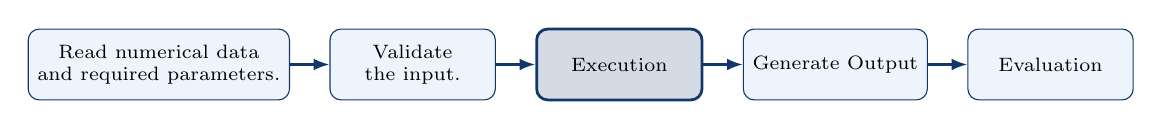
\begin{tikzpicture}[
node distance=5mm,
box/.style={rectangle,rounded corners,draw=GEUBlue,fill=GEULightBlue,
minimum width=2.10cm,minimum height=9mm,align=center,font=\scriptsize},
newbox/.style={rectangle,rounded corners,draw=GEUBlue,fill=GEUBlue!18,line width=1pt,
minimum width=2.10cm,minimum height=9mm,align=center,font=\scriptsize},
arrow/.style={-{Latex[length=2mm]},thick,draw=GEUBlue}
]
\node[box] (a) {Read numerical data \\and required parameters.};
\node[box,right=of a] (b) {Validate \\the input.};
\node[newbox,right=of b] (c) {Execution};
\node[box,right=of c] (d) {Generate Output};
\node[box,right=of d] (e) {Evaluation};
\draw[arrow] (a)--(b);
\draw[arrow] (b)--(c);
\draw[arrow] (c)--(d);
\draw[arrow] (d)--(e);
\end{tikzpicture}
\end{center}

\vspace{3mm}

\begin{columns}[T,totalwidth=\textwidth]
\column{.48\textwidth}
\textbf{\color{GEUBlue}Major Components}
\begin{itemize}\itemsep2pt
\footnotesize
\item Input Handling: Accepts numerical data and parameters, with CSV-reading support
\item Algorithm Classes: Perform the calculations for all algorithms.
\item Output Handling:Evaluation measures where implemented. \emph
\item Main Menu: Displays the available algorithms and accepts the user’s choice.
\end{itemize}

\column{.48\textwidth}
\textbf{\color{GEUBlue}Changes Since Phase-I}
\begin{itemize}\itemsep2pt
\footnotesize
\item C++ classes replace the proposed C modules.
\item Each program contains its own supporting functions and CSV-reading code.
\item Integrated all six algorithms into a single menu-driven application.
\end{itemize}
\end{columns}
\end{frame}

% ============================================================
% SLIDE 6 - MODULE DESIGN
% ============================================================
\begin{frame}[shrink=15]{Module Design \& Functional Requirements}
\begin{columns}[T,totalwidth=\textwidth]
\column{.48\textwidth}
\textbf{\color{GEUBlue}Major Modules}
\begin{enumerate}\itemsep3pt
\footnotesize
\item Linear Regression: Fit a straight line and predict numerical values.
\item SVM: Classify data using a linear decision boundary.
\item KNN: Predict a class from the nearest training examples.
\item K-Means: Group data around cluster centroids.
\item Hierarchical Clustering: Form groups through successive cluster merges.
\item PCA: Reduce dimensionality using principal components.
\end{enumerate}

\column{.48\textwidth}
\textbf{\color{GEUBlue}Functional Requirements}
\begin{itemize}\itemsep3pt
\footnotesize
\item Display a menu containing all six algorithms.
\item Call the appropriate module based on the user’s choice.
\item Accept the required data and parameters.
\item Perform calculations and display readable results.
\end{itemize}
\end{columns}

\vspace{2mm}

\begin{block}{Module Dependency}
\footnotesize
The main program provides a common entry point. Each algorithm retains its own class and calculation functions.
\end{block}
\end{frame}

% ============================================================
% SLIDE 7 - TECH STACK
% ============================================================
\begin{frame}[shrink=15]{Technology Stack \& Development Methodology}
\begin{columns}[T,totalwidth=\textwidth]
\column{.48\textwidth}
\begin{block}{Technology Stack}
\footnotesize
\begin{itemize}\itemsep2pt
\item Programming: Programming Language: C++
\item Development Environment: VS Code
\item Interface: Console-based menu
\item Implementation: Algorithm classes and numerical operations
\item Dataset Format: CSV where supported
\item Version Control: Git and GitHub
\item Planned Reference Validation: Python and Scikit-learn
\end{itemize}
\end{block}

\column{.48\textwidth}
\begin{block}{Development Methodology}
\begin{enumerate}\itemsep2pt
\item Study each algorithm’s mathematics.
\item Design its class and required functions.
\item Implement the algorithm from scratch.
\item Connect the implementation to the main menu.
\item Prepare datasets and validate outputs.
\item Document results and resolve errors.
\end{enumerate}
\end{block}
\end{columns}


\end{frame}

% ============================================================
% SLIDE 8 - PBL CONCEPTS
% ============================================================
\begin{frame}{Implementation of PBL Course Concepts}
\scriptsize
\begin{center}
\renewcommand{\arraystretch}{1.3}
\begin{tabularx}{.96\textwidth}{@{}>{\bfseries}p{2.4cm}X p{2.9cm}@{}}
\toprule
Course & Concepts Implemented & Project Module\\
\midrule
Data Structures in C &
Arrays, array traversal, searching and sorting concepts, numerical accumulation &
Data storage and calculations in Linear Regression and KNN\\
OOPs with C++ &
Classes, objects, constructors, encapsulation, member functions, file handling &
Algorithm classes, CSV input functions, and integrated application\\
\bottomrule
\end{tabularx}
\end{center}

\vspace{3mm}

\begin{center}
\colorbox{GEULightBlue}{\parbox{.88\textwidth}{\centering\footnotesize
\textbf The integrated menu provides access to all six algorithm classes. Each class performs its own calculations and produces the corresponding output.}}
\end{center}
\end{frame}

% ============================================================
% SLIDE 9 - PROGRESS
% ============================================================
\begin{frame}[shrink=15]{Development \& Implementation Progress}
\scriptsize
\begin{center}
\renewcommand{\arraystretch}{1.3}
\begin{tabularx}{.96\textwidth}{@{}p{3.6cm}p{1.8cm}X@{}}
\toprule
\textbf{Module} & \textbf{Status} & \textbf{Work Completed}\\
\midrule
Linear Regression & Completed & Algorithm
implementation\\ 
SVM &	Completed	& Algorithm implementation\\
KNN	&Completed	&Algorithm implementation\\
K-Means	&Completed	&Algorithm implementation\\
Hierarchical Clustering&	Completed	&Algorithm implementation \\
PCA	&Completed	&Algorithm implementation\\
Menu-driven application&	Completed&	Integration of all six algorithms\\
CSV datasets and validation	&Pending	&Dataset preparation and subsequent testing remain\\
\bottomrule
\end{tabularx}
\end{center}

\vspace{3mm}
\begin{center}
\colorbox{GEULightBlue}{\parbox{.65\textwidth}{\centering
\textbf{Overall Project Completion:} approximately 75\%}}
\end{center}
\end{frame}

% ============================================================
% SLIDE 10 - PROTOTYPE
% ============================================================
\begin{frame}{Working Prototype and Demonstration}

\begin{columns}[T,totalwidth=\textwidth]
\column{.45\textwidth}
\textbf{\color{GEUBlue}Features to Demonstrate}
\begin{itemize}\itemsep2pt
\footnotesize
\item Selection of all six algorithms through the main menu
\item Linear Regression predictions and training Mean Squared Error
\item SVM and KNN classification results
\item K-Means and Hierarchical Clustering outputs
\item PCA transformed data
\end{itemize}

\column{.51\textwidth}
\begin{block}{Prototype Output}
\centering
\vspace{4mm}
\fillme{paste a console screenshot here}
\vspace{2mm}

{\scriptsize\color{GEUGrey}Suggested capture: one emergency admission showing the triage order, the bed assigned, and the generated route.}
\vspace{4mm}
\end{block}
\end{columns}
\end{frame}

% ============================================================
% SLIDE 11 - TESTING
% ============================================================
\begin{frame}[shrink=15]{Testing, Results \& Validation}
\scriptsize
\begin{center}
\renewcommand{\arraystretch}{1.3}
\begin{tabularx}{.96\textwidth}{@{}p{2.3cm}X X p{1.3cm}@{}}
\toprule
Test or Module & Expected Result & Observed Result & Status\\
\midrule
Linear Regression &	Correct fitted equation and numerical predictions	Earlier prototype results recorded in the report	&Performed on small data sets& Pending\\
SVM	&Class predictions for labelled inputs	&Performed on small data sets	&Pending\\
KNN	&Class prediction based on nearest-neighbour voting	&Performed on small data sets\\
K-Means	&Cluster assignments and centroid values	&Performed on small data sets	&Pending\\
Hierarchical Clustering	&Grouping through successive cluster merges&	Performed on small data sets&Pending\\
PCA	&Reduced-dimensional representation of numerical data	&Performed on small data sets	&Pending\\
\bottomrule
\end{tabularx}
\end{center}

\vspace{2mm}
\begin{block}{Validation Approach}
\footnotesize
Prepare suitable datasets and compare the outputs with known answers. Validate results against Scikit-learn using comparable settings. The report records nine checks for the earlier Linear Regression prototype; these do not represent testing of all six current implementations.
\end{block}
\end{frame}

% ============================================================
% SLIDE 12 - GITHUB
% ============================================================
\begin{frame}[shrink=15]{GitHub Repository \& Development Activity}

\begin{columns}[T,totalwidth=\textwidth]
\column{.46\textwidth}
\textbf{\color{GEUBlue}Repository Information}
\begin{itemize}\itemsep2pt
\footnotesize
\item GitHub link: {\scriptsize\texttt{github.com/Shubhangani-Kotiyal/PBL-ml-algorithms-in-c}}
\item README.md: Project overview,Menu Driven Program,Dataset Csv File.
\item Contributors: all three members added
\item Branches: \texttt{main}
\end{itemize}

\column{.50\textwidth}
\textbf{\color{GEUBlue}Development Activity}
\begin{itemize}\itemsep2pt
\footnotesize
\item Each member contributes through their own GitHub account.
\item Members work on their assigned algorithm modules.
\item The main program integrates the six algorithms through a menu. \texttt{main}
\item Validation remain pending.
\end{itemize}
\end{columns}

\vspace{1mm}
\begin{center}
\colorbox{GEULightBlue}{\parbox{.88\textwidth}{\centering
\textbf{Requirement:} All team members must be contributors and must
\textbf{commit individually using their own GitHub accounts}.}}
\end{center}
\end{frame}

% ============================================================
% SLIDE 13 - INDIVIDUAL CONTRIBUTION
% ============================================================
\begin{frame}{Individual Contribution}
\scriptsize
\begin{center}
\renewcommand{\arraystretch}{1.4}
\begin{tabularx}{.96\textwidth}{@{}p{2.5cm}p{1.8cm}X p{1.4cm}@{}}
\toprule
Member & Role & Technical Contribution & Commits\\
\midrule
Shubhangani Kotiyal	&Team Lead	&Linear Regression and KNN implementations	& 5\\
Ishanaya Agarwal	&Developer&	SVM and K-Means implementations	& 7\\
Harshita Joshi &	Developer	&Hierarchical Clustering and PCA implementations&	5\\
\bottomrule
\end{tabularx}
\end{center}

\vspace{3mm}
\begin{block}{Individual Evaluation}
\footnotesize
Every member is prepared to explain and demonstrate their own technical contribution.
\end{block}
\end{frame}

% ============================================================
% SLIDE 14 - CHALLENGES & ROADMAP
% ============================================================
\begin{frame}[shrink=15]{Challenges, Remaining Work \& Phase-III Roadmap}

\begin{columns}[T,totalwidth=\textwidth]
\column{.48\textwidth}
\textbf{\color{GEUBlue}Challenges Faced}
\begin{itemize}\itemsep1pt
\footnotesize
\item Converting the C-oriented proposal into a C++ class-based implementation
\item Handling invalid inputs and special calculation cases
\item Completing dataset-based testing and validation
\end{itemize}

\vspace{1.5mm}
\textbf{\color{GEUBlue}Solutions Adopted}
\begin{itemize}\itemsep1pt
\footnotesize
\item Organized the algorithms into separate C++ classes.
\item Added input checks where implemented.
\item Connected all six algorithms through an integrated menu.
\end{itemize}

\column{.48\textwidth}
\textbf{\color{GEUBlue}Remaining Work -- Weekly Plan to 1 Nov}
\begin{enumerate}\itemsep1pt
\footnotesize
\item \textbf{Wk 1} Execute all six algorithms using suitable data.
\item \textbf{Wk 2} Record expected and observed results.
\item \textbf{Wk 3} Compare outputs with Scikit-learn.
\item \textbf{Wk 4} Resolve errors and update documentation.
\end{enumerate}

\vspace{1mm}
{\scriptsize\color{GEUGrey}Phase III: Complete dataset-based validation and prepare the final demonstration of the integrated application.}
\end{columns}
\end{frame}

% ============================================================
% SLIDE 15 - OUTCOMES & REFERENCES
% ============================================================
\begin{frame}[shrink=15]{Expected Outcomes \& References}

\begin{columns}[T,totalwidth=\textwidth]
\column{.47\textwidth}
\textbf{\color{GEUBlue}Expected Final Outcomes}
\begin{itemize}\itemsep2pt
\footnotesize
\item Six machine learning algorithms implemented from scratch in C++
\item An integrated menu-driven application
\item Readable predictions, clustering results, and transformed data
\item Tested results supported by suitable datasets
\item Documentation explaining mathematics, implementation, and execution
\end{itemize}

\column{.47\textwidth}
\textbf{\color{GEUBlue}References}
\begin{enumerate}\itemsep2pt
\footnotesize
\item Bishop, C. M. — Pattern Recognition and Machine Learning
\item Hastie, T., Tibshirani, R., and Friedman, J. — The Elements of Statistical Learning
\item \emph{Stroustrup, B. — The C++ Programming Language}
\begin{figure}
    \centering
    \includegraphics[width=0.5\linewidth]{graphicera_logo.png}
    \caption{Enter Caption}
    \label{fig:placeholder}
\end{figure}
\item Cortes, C., and Vapnik, V. — Support-Vector Networks
\item Scikit-learn Documentation
\end{enumerate}

\vspace{2mm}
\begin{center}
\colorbox{GEUBlue}{\parbox{.78\textwidth}{\centering\color{white}
\textbf{Thank You}\\
Questions \& Suggestions}}
\end{center}
\end{columns}
\end{frame}

\end{document}
